% Do NOT change this "Section" title
% and do NOT add more "Section" level titles.
\section{Implementation}\label{sec:implementation}
This section covers the implementation of all the components making up the mission control system for Naiad.
% You can use how many "subsections" and "subsubsections" you like.
\subsection{Hardware}
It was established early on that the system was going to be run on a BeagleBone Black \cite{web:mcsbbb} board. This allowed the mission control system to be developed using a less stripped down version of Ada, which in the author's oppinion facilitates the development. Limited versions of Ada, for instance the version used on the AT90CAN128 \cite{web:mcsatcan} cards, don't support object oriented language features.

\subsection{Virtual machine}
The virtual machine was implemented to interpret stack machine code. Instructions are read and executed from a binary object file, which makes the interpreter perform operations on
a memory stack.

\subsection{Toolchain for creating missions}
The stack machine code is difficult for a person to read and understand, so the system was designed to have different levels of source code. On the lowest level there is
stack machine code. One level up is a language similar to Ada, which has been named NaiAda (see \cref{sec:naiada}). The highest level is Extensible Markup Language (XML), which is used to aggregate different NaiAda source code files
to create an entire mission which can then be turned into stack machine code. An overview of the toolchain can be seen in \cref{fig:another_column_figure}.

\pageref{fig:another_column_figure}.
\begin{figure}[h]
    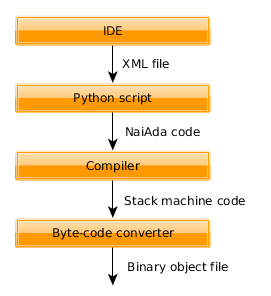
\includegraphics[width=0.5\textwidth]{./figure/figureMissionCreationToolchain.png}
    \caption{The toolchain for creating missions. The arrow captions denodes the output from each step.}
    \label{fig:another_column_figure}
\end{figure}


\subsubsection{Integrated development environment}
The integrated development environment is a graphical application written in Java. It is essentially a drag-and-drop graphical programming application, which allows the user to program entire missions by stringing together different components. The output from the IDE is an XML file, containing all the components of the mission and directions where the source code for each component can be found.

\subsubsection{Aggregator}
The next part in the toolchain is a python script which aggregates the source code for each component of the mission and puts everything in one file containing only NaiAda source code. The aggregation script also inserts a collection of basic NaiAda functions from a single file, which can be used by any primitive. These functions have collectively been called the standard library. This library can be expanded at any time by adding more functions to the same file.

\subsubsection{Compiler}
The compiler's purpose is to translate NaiAda source code into stack machine code. It has been developed in C, using the tools Flex \cite{web:mcsflex} and Bison \cite{web:mcsbison}. Flex is a tool for creating a lexical analyser to use as a scanner for a compiler. Bison is a tool for creating compilers, which can use scanners created with Flex. The compiler has been designed to report errors as precisely as possible. In order to do this, the compiler has different passes.

\begin{description}
\item[Syntax analysis:] This pass checks to see that the syntax is correct according to NaiAda's grammar, which is presented in \cref{sec:grammar}.
\item[Name analysis:] This pass checks to see that all the names for variables, functions and labels are not defined more than once nor undefined.
\item[Type analysis:] This pass checks to see that the types matches up for all the functions, variables and constants.
\end{description}

If any of these passes produces an error, the kind of error will be described in an accurate way pointing to a specific line in the source code. The output from the compiler is a textfile with stack machine code.

\subsubsection{Byte-code converter}
The final step is the byte-code converter, which is used to convert the stack machine code to a binary object file. The motivation for this conversion is the decrease in filesize, and the fact that it is easier for the virtual machine to read binary structures instead of parsing string data.


\subsection{NaiAda}
\label{sec:naiada}
NaiAda is the language the author created to write primitives (see \cref{sec:primitives}) in. It is designed to be as close to Ada as possible, and has been developed to have the ability to do everything you would want the AUV to do.
\subsubsection{Types}
\begin{description}
\item[Boolean:] This type has two values, true or false.
\item[Integer:] This type represents integers.
\item[Float:] This type represents decimal numbers.
\item[Vector:] This type represents vectors in 3D space.
\item[Matrix:] This type represents 3x3 matrices in 3D space.
\end{description}

\subsubsection{Access types}
Any variable can be pointed to using access types. This allows for functions to change the values of variables outside scope.

\subsubsection{Functions and procedures}
Functions and procedures work the same way as they do in Ada. The difference between them are that functions can return a value whereas procedures can not.

\subsubsection{Labels}
Labels were included in the language to enable the IDE to branch the execution path. A branch in the IDE makes the aggregator produce goto-statements in the NaiAda code.

\subsubsection{Typecasting}
Typecasting exists in the language to convert from float to integer and from integer to float.

\subsubsection{Basic statements}
The language features a couple of basic statements which basically works the same way as they do in Ada.
\begin{description}
\item[if-then-else:] Allows the execution path to branch.
\item[while-loop:] Allows the execution to loop as long as a specified condition is true.
\end{description}

\subsubsection{Basic math functionality}
Some basic math functionality has been implemented in the language. The math functions that are native in NaiAda are:
\begin{description}
\item[sin:] Calculates the sine value for an angle.
\item[cos:] Calculates the cosine value for an angle.
\item[arcsin:] Calculates the angle from a sine value.
\item[arccos:] Calculates the angle from a cosine value.
\item[abs:] Returns the absolute value for a value.
\item[sqrt:] Calculates the square root of a value.
\end{description}


